% Created 2021-03-30 Tue 13:19
% Intended LaTeX compiler: pdflatex
\documentclass[11pt]{article}
\usepackage[utf8]{inputenc}
\usepackage[T1]{fontenc}
\usepackage{graphicx}
\usepackage{grffile}
\usepackage{longtable}
\usepackage{wrapfig}
\usepackage{rotating}
\usepackage[normalem]{ulem}
\usepackage{amsmath}
\usepackage{textcomp}
\usepackage{amssymb}
\usepackage{capt-of}
\usepackage{hyperref}
\usepackage[margin=30mm]{geometry}
\date{2021 March 26}
\title{TAB2XML Design Document\\\medskip
\large For version 0.4.0}
\hypersetup{
 pdfauthor={},
 pdftitle={TAB2XML Design Document},
 pdfkeywords={},
 pdfsubject={},
 pdfcreator={Emacs 27.1 (Org mode 9.4.4)}, 
 pdflang={English}}
\begin{document}

\maketitle
\tableofcontents

\newpage

\section{Front End Design}
\label{sec:org5c26d21}
\emph{All TAB2XML front-end code is located in the \texttt{tab2xml.gui} package.}
\subsection{Front End Classes}
\label{sec:org66eb0f0}
\begin{figure}[htbp]
\centering
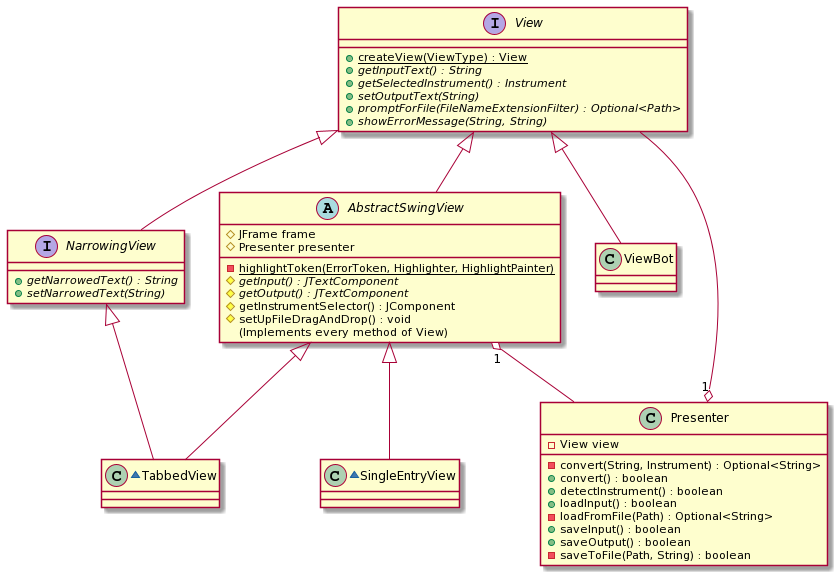
\includegraphics[width=.9\linewidth]{./Diagrams/frontend-class-diagram.png}
\caption{A class diagram for the frontend of TAB2XML.}
\end{figure}

The frontend of TAB2XML is designed using the \href{https://en.wikipedia.org/wiki/Model\%E2\%80\%93view\%E2\%80\%93presenter}{MVP} paradigm.  It is divided into two main parts, the \texttt{View} and the \texttt{Presenter}.

The \texttt{View} is the part of the frontend that interacts with the user (the GUI).  It is handled by the \texttt{View} interface; the GUIs for TAB2XML implement the View interface.  In addition, all Views that represent a Swing GUI are subclasses of the skeletal implementation \texttt{AbsractSwingView}, which reduces the effort needed to make a View.  Currently, there are four concrete classes implementing \texttt{View}: \texttt{TabbedView} (currently the one in use), \texttt{SingleEntryView}, \texttt{DoubleEntryView} and \texttt{ViewBot} (a mock view used for testing).  The \texttt{NarrowingView} interface represents Views that additionally support TAB2XML's tab-narrowing functionality.

The \texttt{Presenter} is the part of the frontend that interacts with the backend code.  It is a single class, not an interface that has multiple implementations.  It implements behaviours such as converting a tab, loading from a file and detecting the instrument of the input tab.  It uses the View interface's public methods to interact with the view.  This means that the View's buttons can simply be linked to call the Presenter's methods, instead of having to implement the method in the View.  All of the Presenter's methods return either a \texttt{boolean} or an \texttt{Optional} to describe whether they succeeded or not.

The rationale behind this design is to reduce the effort involved in creating a new GUI.  If it extends \texttt{AbstractSwingView}, creating a new View is as simple as making a "mockup" Swing GUI and implementing two trivial methods.  This makes it easy to work with multiple GUIs at once (allowing the customer to choose which they prefer).  This design was especially important in the beginning of development, because I could prototype different GUI ideas with the customer using fully functional applications.
\subsection{Converting Text Tabs}
\label{sec:orga5f50ca}
\begin{figure}[htbp]
\centering
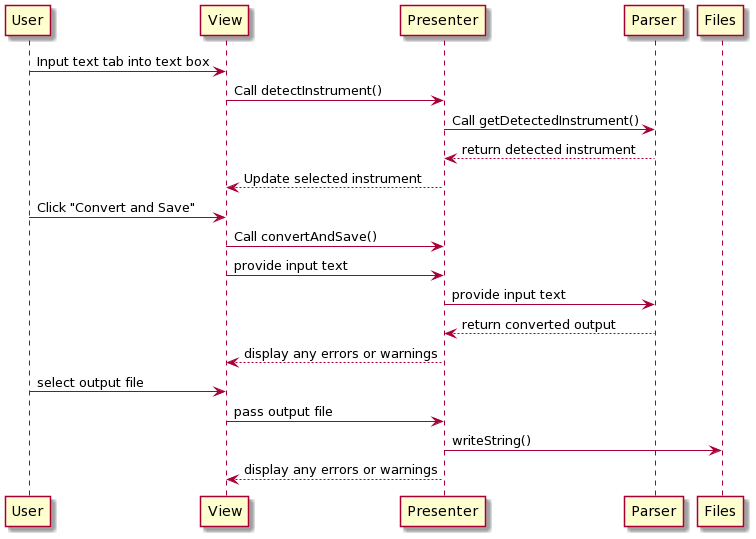
\includegraphics[width=.9\linewidth]{./Diagrams/convert-and-save.png}
\caption{A sequence diagram for the "Convert and Save" operation}
\end{figure}

Here is how the "Convert and Save" operation works:
\begin{enumerate}
\item The user inputs the tab into the input text box (by typing, copy-and-pasting, the "Load from File" button or dragging and dropping a file).
\item The \texttt{View} calls the backend method \texttt{Parser.getDetectedInstrument(String)} with its text as input.
\item If it succeeded, the \texttt{View} sets its selected instrument to the detected instrument.
\item The user clicks the "Convert and Save" button.
\item The \texttt{View} calls the \texttt{Presenter}'s \texttt{convertAndSave()} method.
\item The \texttt{Presenter} calls the \texttt{View}'s \texttt{getInputText()} and \texttt{getSelectedInstrument()} methods to get the input tab and selected instrument.
\item The \texttt{Presenter} creates a new instance of \texttt{Parser} with the obtained input text and instrument.  It then calls the \texttt{Parser}'s \texttt{parse()} method to convert the text tab.
\item The \texttt{Parser} returns the MusicXML, as well as any errors that occurred.  Critical errors are thrown as Exceptions, noncritical errors are returned.  This distinction exists so that critical errors stop the parsing, while noncritical errors do not stop it.
\item The \texttt{View} displays any errors or warnings to the user.
\item The \texttt{Presenter} calls the \texttt{View}'s \texttt{promptForFile} method to prompt the user for the desired destination file.
\item The \texttt{Presenter} calls \texttt{Files.writeString} to write the text tab to the selected file.
\item The \texttt{View} displays any errors that occurred during the file-saving operation.
\end{enumerate}
\subsection{Front End Maintenance}
\label{sec:orgbaeb792}
To create a new GUI, simply make your GUI handled by a class that extends \texttt{View}.  It should also have a \texttt{Presenter} field instantiated using \texttt{new Presenter(this)}.  You must implement all of the \texttt{View}'s methods, which is much easier if you extend \texttt{AbstractSwingView}.  Then, you can call the presenter's methods within the GUI, and your GUI will be fully connected to the TAB2XML backend.

To modify the look of an existing View such as \texttt{TabbedView} (or add/remove components), simply modify its constructor (you may have to edit the other methods, if they are broken by the change).  If you are adding a new feature that should exist in every Swing View, consider instead adding it to \texttt{AbstractSwingView}, as this will make it available for every View.
\end{document}
